\chapter{\IfLanguageName{dutch}{Stand van zaken}{State-of-the-art}}%
\label{ch:standvanzaken}

Gezichtsanalyse bestaat uit het definiëren van menselijke gezichten in real time, met behulp van computeralgoritmen en machine learning technieken. Voor mensen en computersystemen bevat een gezichtsbeeld details zoals leeftijd, geslacht, stemming, afkomst, et cetera. \\
\\ 
Gezichtsanalyse omvat dan ook het lokaliseren en meten van gezichtskenmerken in een afbeelding. Vervolgens wordt het gezichtsbeeld geanalyseerd voor het extraheren van kenmerken \autocite{Sanil2023}. Gezichtsanalyse speelt dan ook een grote rol in real world applicaties, zoals animatie, identiteitsverificatie, medische diagnose, et cetera. Ondanks het bestaande onderzoekswerk over dit onderwerp, is gezichtsanalyse nog steeds een lastige taak vanwege verschillende factoren zoals veranderingen in hoek, gezichtsuitdrukkingen en achtergrond \autocite{Siddiqi2022}. \\
\\
Volgens onderzoek van \textcite{Basystiuk2023} is beeldherkenning een simpele procedure die uit slechts 3 stappen bestaat. 
\begin{enumerate}
    \item Preprocessing: We voegen filters toe aan de afbeelding om het geschikter te maken voor herkenning.
    \item Feature Extractie: We identificeren belangrijke data en behouden deze om mee verder te werken. Dit wordt verder besproken in \ref{sub:gezichtsdetectie}.
    \item Classificatie: het analyseren en identificeren van de data na de feature extractie.
\end{enumerate}


\section{Gezichtsdetectie}\label{sub:gezichtsdetectie}
Gezichtsdetectie is de eerste stap in het bepalen van de gezichtsfeatures. Deze features zijn de interessante delen van het gezicht , bijvoorbeeld ogen, neus en mond en worden ook wel eens landmarks genoemd \autocite{Coppens2018}. In dit onderzoek raadt de auteur 3 gezichtsdetectieservices aan: Microsoft Face API, Face++ en Kairos. Deze zijn alle 3 ook geschikt om geslacht en leeftijd te voorspellen. Er wordt met 3 services tegelijk gewerkt om elkaars beperkingen op te vangen.
In het onderzoek van \textcite{Sanil2023} berekenen ze de landmarks op 2 verschillende methoden: Euclidische afstand en Geodetische afstand. \\

\textcite{Sanil2023} stelt 468 landmarks visueel voor, in plaats van 68, om de accuracy te verbeteren. Dit door gebruik te maken van de Mediapipe library (\textcite{Zubair2021}). Op figuur {~\ref{fig:landmarks}} staan de belangrijkste antropometrische landmarks aangeduid . Het is noodzakelijk om de belangrijkste features te identificeren die kunnen leiden tot het correct voorspellen van de leeftijd of het geslacht. Om de leeftijd te voorspellen kunnen we bijvoorbeeld de rimpels op de gezichtsfoto analyseren \autocite{Kwon1994}. 
\begin{figure}
    \centering
    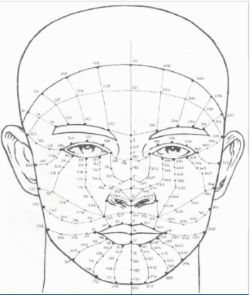
\includegraphics{graphics/faciallandmarks.png}
    \caption[Belangrijkste anthropometrische landmarks]{De belangrijkste anthropometrische landmarks\autocite{Sanil2023}.
    \label{fig:landmarks}}
\end{figure}


\section{Feature extractie} \label{sec:featextractie}
\subsection{Normalisatie}\label{sub:normalisatie}
In onderzoek van \autocite{Chen2011} voor het voorspellen van leeftijd op basis van afbeeldingen werden de gezichtsafbeeldingen genormaliseerd voor de feature extractie plaatsvond. De geometrie van de afbeeldingen kan worden genormaliseerd op basis van de gedetecteerde features, zoals oog of mond coördinatie. De auteur maakt gebruik van een mask om de pixels die zich niet in de ovaal van de typsiche gezichtsregio bevinden te verwijderen. Dit gaat dan bijvoorbeeld over haar en hemdskragen. Zo blijven enkel de belangrijkste features van het gezicht over. Figuur {~\ref{fig:beforenormalisation}} geeft een voorbeeld van een dataset met gezichtsfoto's. In figuur {~\ref{fig:afternormalisation}} worden deze afbeeldingen genormaliseerd, waardoor er minder variaties overblijven in de afbeeldingen en we bijvoorbeeld al geen achtergrond overhouden.
\begin{figure}
    \centering
    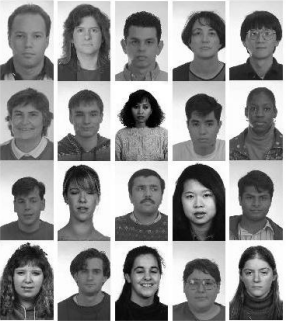
\includegraphics{graphics/beforenorm.PNG}
    \caption[Gezichtsafbeeldingen voor normalisatie]{Gezichtsafbeeldingen voor normalisatie\autocite{Chen2011}.
        \label{fig:beforenormalisation}}
\end{figure}
\begin{figure}
    \centering
    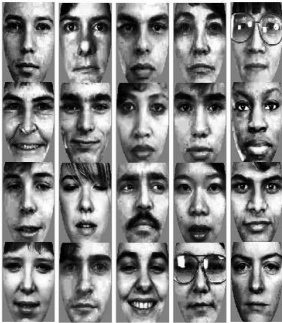
\includegraphics{graphics/afternorm.PNG}
    \caption[Gezichtsafbeeldingen na normalisatie]{Gezichtsafbeeldingen na het toepassen van normalisatie\autocite{Chen2011}.
        \label{fig:afternormalisation}}
\end{figure}  \\
De gezichtsafbeeldingen kunnen ook genormaliseerd worden op basis van de coördinaten van de ogen, zodat het centrum van beide ogen van de afbeeldingen op een vaste positie liggen \autocite{Chen2011}. 

\subsection{AAM}\label{sub:aam}
In het onderzoek van \textcite{Lakshmiprabha2016} worden de Active Appearance Model (AAM) features gebruikt in de feature extractie stap. Deze features zijn geschikt om het effect van veroudering weer te geven voor het voorspellen van geslacht. De features die we van AAM krijgen hebben zowel vorm- als textuurinformatie die geschikter is voor veroudering. Figuur {~\ref{fig:aam}} geeft een representatie van de FG-NET database na het toepassen van de AAM-features. Het resultaat is vergelijkbaar met de normalisatie van \textcite{Chen2011} op figuur {~\ref{fig:afternormalisation}}.
\begin{figure}
    \centering
    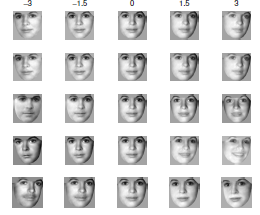
\includegraphics{graphics/AAM.PNG}
    \caption[AAM-features]{Cohn Kanada database na toepassen van AAM \autocite{Lakshmiprabha2016}.
        \label{fig:aam}}
\end{figure} 

\subsection{LBP} \label{sub:lbp}
Local Binary Patterns (LBP) is een textuurdescriptor die gebruikt kan worden om gezichten te representeren, aangezien een gezichtsfbeelding kan worden beschouwd als een samenstelling van microtextuurpatronen \autocite{SanchezLopez2010}. De LBP operator kent een label toe aan elke pixel van een afbeelding door een threshold te nemen van de 3x3 buren met de centrale piwelwaarde en het resultaat te beschouwen als een binair getal. Het resultaat na de toepassing van LBP in het onderzoek van \textcite{SanchezLopez2010} is weergegeven op figuur {~\ref{fig:lbp}}.
\begin{figure}
    \centering
    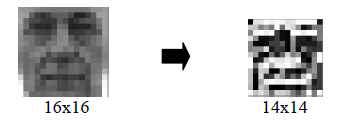
\includegraphics{graphics/LBP.PNG}
    \caption[AAM-features]{Toepassen van LBP op een 16x16 gezichtsafbeelding resulteert in 14x14 label afbeelding \autocite{SanchezLopez2010}.
        \label{fig:lbp}}
\end{figure}
\\
In het onderzoek van \textcite{Chen2011} wordt LBP toegepast om de gezichtsfeatures te extraheren uit elk blok die de leeftijdsinformatie bevat. Het resultaat hiervan is een feature dimensie vector van 59. Deze features worden dan samengevoegd in een holistische vector. 

\subsection{HOG features} \label{sub:hog}
Histograms of Oriented Gradients (HOG) begint met het tellen van de oriëntatie van de gradiënten in gelokaliseerde delen van een afbeelding. De afbeelding wordt verdeeld in kleine verbonden gebieden, genaamd cellen, en voor elke cel wordt een
histogram van gradiëntrichtingen of randoriëntaties voor de pixels binnen de cel gecompileerd \autocite{Deniz2011}. \\
De HOG features worden exclusief gebruikt voor gezichtsdetectie. De features die uit de omgeving van de landmarks in het gezicht worden gehaald, worden gebruikt voor classificatie en maken gebruik van het nearest neighbour algoritme en de Euclidische afstand. \\
\\
\textcite{Tomasi2015} gebruikt de HOG features om menselijke voetgangers te detecteren. Figuur {~\ref{fig:hog}} geeft de extractie van de HOG features uit een afbeelding weer. 
\begin{figure}
    \centering
    \includegraphics{graphics/hog.PNG}
    \caption[HOG features]{Toepassen van HOG op een gezichtsafbeelding \autocite{Tomasi2015}.
        \label{fig:hog}}
\end{figure}

\section{Feature dimensionaliteitsreductie} \label{sec:featuredimred}
De herkenning van gezicht focust zich voornamelijk op het detecteren van individuele features in het gezicht, zoals ogen, hoofdomtrek, mond of het definiëren van het model van gezicht door positie, grootte of relatie tussen de features \autocite{Lin2006}. Het extraheren van de features speelt een grote rol in de preprocessing fase. \\
\\

\subsection{PCA} \label{sub:PCA}
De Principal Component Analyse (PCA) wordt veelal gebruikt voor gezichtsherkenning. PCA is een unsupervised, statistische techniek die gebruikt wordt voor dimensionaliteitsreductie in machine learning \autocite{SalihHasan2021}. Het reduceert het hoge aantal dimensies in een grote dataset naar een lager aantal dimensies om de opslag en het verwerkingsproces te versnellen. Hierdoor is de data makkelijker te interpreteren en sneller te verwerken. De techniek behoudt het grootste aantal informatie en verwijdert redundante ruis en data. Het grote nadeel van PCA is dat de lineaire transformatie die wordt uitgevoerd om de grootste varianties te behouden, niet altijd goed geschikt is voor het op te lossen probleem, namelijk de classificatie van geslacht \autocite{Wang2010}. \\
De feature reductie vindt typisch plaats na de feature extractie fase en voor de eigenlijke classificatie \autocite{Lakshmiprabha2016}.
\\
\subsection{Truncated SVD} \label{sub:truncatedsvd}
De Truncated singular value decomposition, ofwel Truncated SVD, is een benaderingsmethode voor lage-rankmatrices die veelal gebruikt wordt in data science, machine learning en lineaire algebra \autocite{Yeh2022}. \\
De benadering van de lage-rankmatrix is een dimensionaliteitsreductie methode die van belang is bij de groeiende hoeveelheid data waar traditionele methoden niet mee kunnen omgaan. Deze lage-matrix benaderingsmethoden benaderen een bepaalde matrix als product van meerdere kleinere matrices en wordt gebruikt om de geheugenkost en tijd die nodig is om de modellen te trainen te verminderen. \\
Truncated SVD is de optimale lage-rank matrix benadering en wordt hierdoor toegepast in machine learning als dimensionaliteitsreductie. PCA is ook een vorm van Truncated SVD, maar hierbij wordt de singulaire waarde, \textit{k}, bepaald met een statistische interpretatie.   

\section{Bestaande uitdagingen} \label{sec:uitdagingen}
Ondanks het uitgebreide onderzoekwerk, heersen er nog vele uitdagingen op het vlak van gezichtsanalyse. Deze uitdagingen zijn het gevolg van verschillende factoren zoals gezichtsuitdrukkingen, ruis, belichting, et cetera. Om de nauwkeurigheid van de gezichtsherkenning te verbeteren, is het belangrijk om taken van de gezichtsanalyse met elkaar te correleren. Het is bijvoorbeeld zeer waarschijnlijk dat mannen een baard of snor kunnen hebben, maar vrouwen en kinderen niet \autocite{Siddiqi2022}. 
\\
Ook is het detecteren van de locatie waar de gezichten zich bevinden op de afbeelding een uitdaging. Dit wordt vaak meegenomen in de preprocessing stap van het analysesysteem \autocite{Jiang2008}.
\\
De problemen situeren zich niet enkel op het vlak van de afbeelding, maar ook bij de machine learning modellen. Eén van de grootste problemen hierbij is overfitting. Dit gebeurt wanneer we het algoritme te veel trainen, waardoor het te hard lijkt op de trainingsdata. Hierdoor zal het systeem falen wanneer we nieuwe data willen classificeren \autocite{Coppens2018}.

\section{Bestaande Machine-Learning technieken} \label{sec:bestaandeml}
Supervised learning is de methode die input mapt naar een output, gebaseerd op een voorbeeld \autocite{Rustam2018}. Supervised learning is gericht op het voorspellen van de waarde van variabelen of labels, op basis van de input features. Het wordt gewoonlijk gebruikt voor classificatie, benadering, modelleren of identificatie. Het groeperen van mannen of vrouwen op basis van gezichtsherkenning is een classificatieprobleem. Er zijn 2 opties: man of vrouw, ofwel 0 of 1. Dit maakt supervised learning de geschikte methode voor de voorspelling van geslacht. Bij supervised learning bestaat de trainingsdata uit een reeks trainingsvoorbeelden, waarbij elk voorbeeld bestaat uit een input en een verwachte output waarde \autocite{Shah2012}. Het algoritme analyseert de trainingsdata en voorspelt dan de correcte output categorie voor de gegeven data input.  

\subsection{Extreme Gradient Boost}
\label{sub:xgboost}
Extreme Gradient Boost, ofwel XGBoost, is een supervised learning model, waar trainingdata, met meerdere features, x\textsubscript{i} wordt gebruikt om target waarde y\textsubscript{i} te voorspellen \autocite{XGBoost2023}. Uit onderzoek van \autocite{Chen2023}, waarbij vermoeidheid werd voorspeld op basis van gezichtsafbeeldingen met XGBoost, wordt een boom aangemaakt op basis van de geleverde features. Dit model gaf een hoge accuracy en is minder gevoelig voor noise. Uit onderzoek naar gezichtsdetectie van \textcite{Sanil2023} bleek dat Extreme gradient boosting de beste resultaten gaf, met een accuracy van 78\%, gevolgd door Adaptive Boosting (77\%) en Random Forest (75\%). 

\subsection{Adaptive Boosting}
\label{sub:adaboost}
De Adaptive Boost, of AdaBoost, is typisch een classificatie tussen twee klassen  \autocite{Guo2001}. Deze ML-techniek kan dus toegepast worden op de voorspelling van man of vrouw (0 of 1). Om het herkenningsprobleem met meerdere klassen op te lossen, kan een majority voting (MV) strategie worden gebruikt om alle paarsgewijze classificatieresultaten te combineren. Hierbij kiezen we de meest voorkomende klasse als voorspelling. AdaBoost is een adaptief algoritme om een reeks classificeerders te boosten, in die zin dat de gewichten dynamisch worden bijgewerkt op basis van de fouten in eerdere leerresultaten.

\subsection{Random Forest Classifier}
\label{sub:randomforest}
Random forests zijn verzamelingen decision trees die elk getraind zijn op een willekeurig gekozen deelverzameling van de beschikbare data. Deze decision trees worden willekeurig door de trainingsvoorbeelden die aan elke boom worden gegeven,  maar ook door een willekeurige subset van tests die beschikbaar zijn voor optimalisatie op elke node \autocite{Fanelli2012}. Wanneer we een input vector aan het model geven, gaat het model bewegen door de gepaste boom \autocite{Chen2011}. De uiteindelijke classificatie is gebaseerd op een majority voting over alle bomen. Uit het onderzoek van \textcite{Wang2010} blijkt dat Random Forest ook geschikt is voor feature selectie. \\
\\
Een voorbeeld voor het gebruik van Random Forest in gezichtsanalyse is figuur {~\ref{fig:randomforest}}. Hierbij wordt een boom getoond voor het  schatten van de houding van het hoofd. 
\begin{figure}
    \centering
    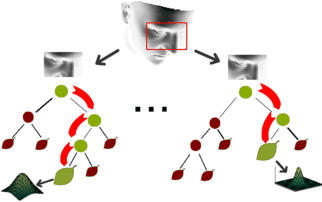
\includegraphics{graphics/headposition.png}
    \caption[Random forest voor houding van het hoofd]{Voorbeeld van een random forest voor het schatten van de houding van het hoofd\autocite{Fanelli2012}.
        \label{fig:randomforest}}
\end{figure} \\
\\
Het onderzoek van \textcite{Mady2018} gebruikt random forest classifier voor de herkenning en detectie van gezichten. De classifier wordt toegepast op het gezicht om dit te herkennen uit de databank. Hier wordt aangehaald wanneer we het aantal bomen in de random forest verhogen, zal ook de nauwkeurigheid verhogen, maar is het ook veel tijdrovender. De random forest is dus een trade-off tussen accuracy en tijd. Het toevoegen van Local Binary Pattern (LBP) en Histogram of Oriented Gradient(HOG) verhoogde de algemene accuracy van de classifier. 

\subsection{Support Vector Machines} \label{sub:svm}
Een Support Vector Machine (SVM) is een ML-techniek die gebruikt wordt voor patroonclassificatie en regressieanalyse \autocite{Chen2011}. Het is gebaseerd op het zoeken naar een lineaire grens tussen twee klassen van patronen. Het SVM mechanisme gaat opzoek naar de optimale classifier die de data in 2 verschillende klassen opdeelt \autocite{Rustam2018}. De optimale classifier wordt de hyperplane genoemd. Dit kunnen we vinden door de marge te maximaliseren en zal zorgen voor zo min mogelijk misclassificatie. \\
\\
Voor niet-lineair scheidbare data mappen we alle punten naar een feature ruimte door gebruik te maken van een kernel \autocite{Shah2012}. Na het splitsen, kunnen we de punten terug mappen naar de input ruimte met een kromme hyperplane, zoals op figuur {~\ref{fig:svm}}. \\
Een SVM is zeer effectief wanneer een hoog aantal dimensionele ruimtes zijn. Ze zijn ook veelzijdig, aangezien we meerdere kernels kunnen gebruiken. De keuze van kernel is afhankelijk van de requirements van het model en heeft een grote invloed op de resultaten van een model. Het voordeel van een SVM model is dat het accurate voorspellingen kan maken, onafhankelijk van de grootte (image size) van de afbeeldingen. \autocite{Khan2011} \\
\\
In het onderzoek van \textcite{Rustam2018} wordt SVM gebruikt voor de classificatie van leeftijdsgroepen en bereikt de maximale accuracy van 100 \%.
\begin{figure}
    \centering
    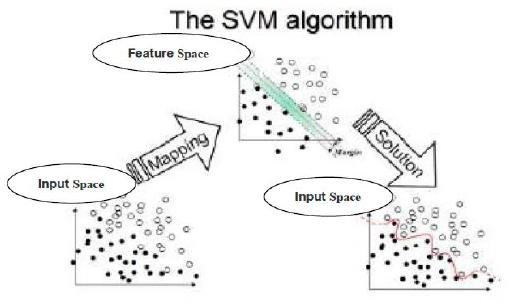
\includegraphics{graphics/svm-non-lineair.PNG}
    \caption[SVM]{Support Vector Machine voor niet-lineair scheidbare data
        \label{fig:svm}}
\end{figure}

\subsection{Logistic Regression}\label{sub:logregression}
Logistische regressie is een populair algoritme voor binaire classificatie taken, zoals voorspellen van geslacht \autocite{Ramon2024}. Het modelleert de relatie tussen de input variabelen en de kans dat de afbeelding tot een bepaalde geslachtscategorie behoort. Logistische regressie gebruikt de logistische funtie om een lineaire combinatie van de features te maken. Dit wordt uiteindelijk gebruikt om voorspellingen te maken. Logistische regressie wordt gebruikt om de kans dat een instantie behoort tot een bepaalde klasse te voorspellen, zoals bijvoorbeeld de classificatie van spam of niet \autocite{Geron2019}. Als de instantie tot de klasse behoort, voorspelt die 1, anders 0. Dit maakt het dus een binaire classifier. 
\\
Het onderzoek van \textcite{Yavuz2014} gebruikt een logistisch regressiemodel om geslacht te voorspellen. Aan het model werden 2 verschillende optimisatiemethoden toegevoegd, namelijk Stochastic Gradient Following (SGF) en limited memory Broyden-Fletcher-Goldfarb-Shanno algoritme (L-BFGS). SGF is efficiënt en makkelijk te implementeren, wat het één van de meest gebruikte optimisatie algoritmes maakt. Doordat het onderzoek van \textcite{Yavuz2014} slechts een beperkte dataset gebruikt, had het L-BFGS model een grotere error rate dan het SGF model. Dit toont nogmaals aan dat een goede dataset belangrijk is. 

\subsection{Ensemble}
\label{sub:ensemble}
Een set van 30 Lineaire Discriminant Analyse (LDA) dienen als basis classifiers en dragen bij tot het ensemble in het model van \textcite{Khan2017}. Het ensemble gebruikt de gecombineerde classificatiecapaciteiten van de base classificiers, zo verbeteren we de algehele prestaties. De volledige pipeline voor de gezichtsanalyse vinden we in figuur {~\ref{fig:ensemble}}. 
\begin{figure}
    \centering
    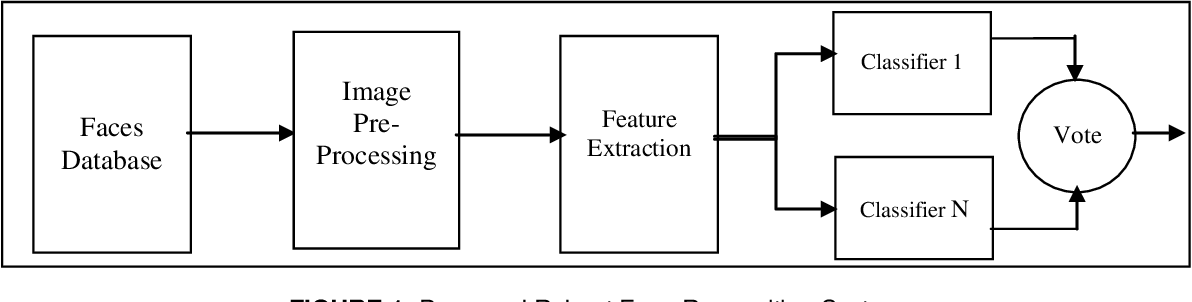
\includegraphics[width=\columnwidth]{graphics/ensemble.png}
    \caption[Robuust gezichtsherkenning systeem]{Robuust Gezichtsherkenning systeem\autocite{Khan2017}.
        \label{fig:ensemble}}
\end{figure}

\subsection{Multi attribution model}\label{sub:mamodel}
In het onderzoek van \autocite{Gupta2022} wordt een multi-attribution model uitgewerkt. Dit voorspelt leeftijd en geslacht door middel van slechts 1 model. Het multi-attribution model voorspelt dus beide: leeftijd en geslacht. Het model van \autocite{Guo2014}, dat gebruik maakt van de Biologically Inspired Feature (BIF), gaf betere resultaten in vergelijking met individuele feature modellen. Een CNN is het meest gebruikte model voor multi-attribution, maar dit valt buiten de scope van deze bachelorproef.

\subsection{Grid Search en Random Search} \label{sub:gridsearch}
Hyperparameters representeren de specifieke parameters die we meegeven aan een Machine Learning model alvorens de training te beginnen \autocite{Ibtisamah2023}. De hyperparameters kunnen worden gefinetuned op verschillende configuraties om het model beter te doen presteren. Het individueel trainen van deze hyperparameters is tijdrovend en daarom kunnen zoekstrategieën gebruikt worden om meerdere hyperparameters tegelijk uit te testen om de meest geschikte eruit te halen. Grid Search en Random Search zijn de bekendste strategieën en zijn beschikbaar gesteld via Scikit-learn \autocite{ScikitLearn2024}. Bij Grid Search geven we verschillende hyperparameters mee, die het model gaat onderzoeken. Bij Random Search geven we een range van hyperparameter waarden mee, wat het efficiënter maakt dan Grid Search.  Grid Search maakt gebruik van cross validatie, waarbij de dataset in willekeurige groepen wordt opgedeeld \autocite{Beheshti2022}. Een testgroep wordt opzij gehouden en de overige groepen worden getraind. Dit proces wordt herhaald tot elke groep testgroep is geweest. Hiervan wordt dan het gemiddelde genomen. De standaardwaarde voor het aantal herhalingen is 5. Figuur ~\ref{fig:crossval} geeft hier een visuele representatie van. 

\begin{figure}[H]
    \centering
    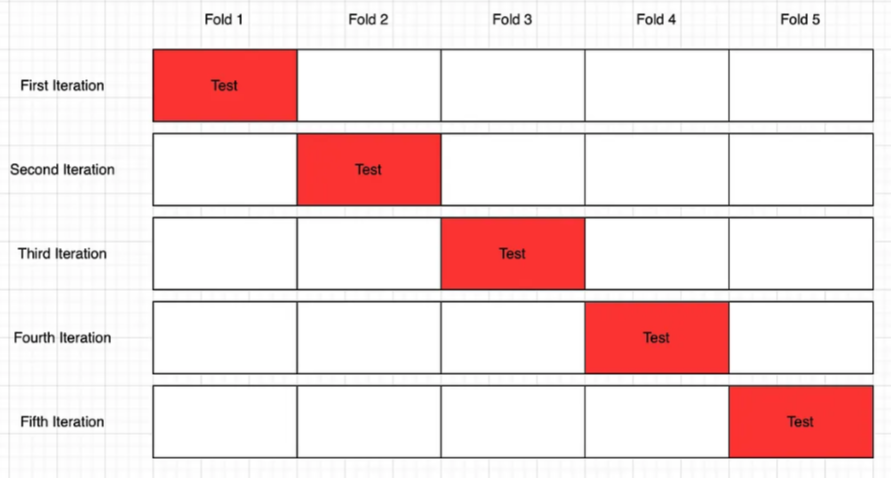
\includegraphics{graphics/gridsearch.png}
    \caption[Cross validatie voor Grid Search]{Cross validatie voor Grid Search \autocite{Beheshti2022}.
        \label{fig:crossval}}
\end{figure}\\

% list and dataset missing
Hieronder een code voorbeeld van hoe \autocite{Educative2024} met behulp van de Grid Search verschillende hyperparameters definieert.
\begin{lstlisting}[style=mystyle, caption={GridSearchCV}]
    from sklearn.model_selection import GridSearchCV, train_test_split
    from sklearn.ensemble import GradientBoostingRegressor
    from sklearn.datasets import load_diabetes
    
    X,y = load_diabetes(return_X_y=True)
    X_train, X_test, y_train, y_test = train_test_split(X, y, test_size=0.33, random_state=42)
    
    % Creating a Model
    model = GradientBoostingRegressor()
    
    % Define the hyperparameter grid
    param_grid = {'learning_rate': [0.2,0.02,0.02,1],
        'max_depth'    : [2,4,6,8,10]
    }
    
    % Create the GridSearchCV object
    grid_search = GridSearchCV(estimator=model, param_grid=param_grid, cv=5, n_jobs = -1)
    
    % Perform the grid search
    grid_search.fit(X_train, y_train)
    
    % Access the best hyperparameters and best score
    best_learning_rate = grid_search.best_params_['learning_rate']
    best_max_depth = grid_search.best_params_['max_depth']
    best_score = grid_search.best_score_
    
    % Print the results
    print("Best learning rate:", best_learning_rate)
    print("Best Depth:", best_max_depth)
    print("Best score (MSE):", best_score)
\end{lstlisting}
% dataset section gives errors

\section{Dataset} \label{sec:dataset}
Uit onderzoek van \textcite{Karkkainen2021} bleek dat bestaande, publieke datasets sterk bevoordeeld zijn naar blanke mensen. Modellen die getraind worden op enkel 1 publieke dataset vertonen dan ook slechte en inconsistente resultaten. Kärkkäinen gebruikt in zijn onderzoek een zelf samengestelde dataset, met 108501 afbeeldingen die verdeeld zijn over elk ras. De resultaten van het onderzoek op de dataset vertonen een betere accuraatheid over verschillende rassen en leeftijdsgroepen. Op figuur {~\ref{fig:datasets}} wordt de verdeling over geslacht en ras van de Fairface dataset die \textcite{Karkkainen2021} gebruikt weergegeven tegenover de UTKFace en LFWA+ dataset. Hieruit is duidelijk dat LFWA+ biased is naar witte mannen en dus niet geschikt is om een accuraat onderzoek uit te voeren. 
\begin{figure}
    \centering
    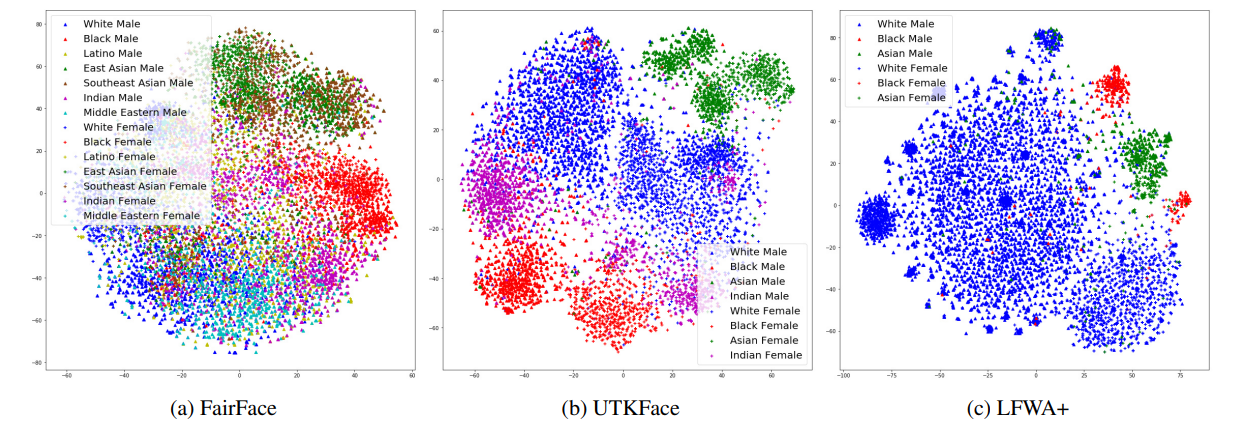
\includegraphics[width=\columnwidth]{graphics/datasets.png}
    \caption[FairFace, UTKFace en LFWA+ datasets]{ FairFace, UTKFace en LFWA+ datasets \autocite{Karkkainen2021}.
        \label{fig:datasets}}
\end{figure}\\
\\
Ook in het onderzoek van \textcite{Buolamwini2018} wordt een eigen dataset aangemaakt. Hier wordt niet enkel gekeken naar ras, maar bijvoorbeeld ook naar dikte en hoeveelheid haar. Het model moet zodoende dezelfde accuraatheid geven over verschillende leeftijdsgroepen, geslachten, rassen, et cetera. Uit het onderzoek bleek ook dat resultaten bij modellen die gebruik maken van Microsoft's Face Detect of Face++ een slechtere precisiescore vertonen, mogelijks door bias in trainingsdata. 
 


\section{Voorspellen van geslacht en leeftijd} \label{sec:voorspellen}
Het eerste baanbrekende onderzoek op het vlak van classificatie op basis van gezichtsafbeeldingen dateert uit 1994. \textcite{Kwon1994} voorspelde in dit onderzoek slechts 3 leeftijdsgroepen: baby's, tieners en volwassen. Het onderzoek focuste zich op het vinden van de primaire features in het gezicht, zoals ogen, mond en neus, en combineerde dit met secundaire features, zoals rimpels. Hiermee toonde het onderzoek aan dat de gezichtsfeatures een grote rol spelen in het classificeren van leeftijd. Dit onderzoek vormt dan ook de basis voor vele verdere onderzoeken op het vlak van classificatie.  \\
\\ 
Menselijke gezichten zijn onderhevig aan veroudering en groei \autocite{Gupta2022}. Deze verandering in uiterlijk kan verschillen van persoon en is het gevolg van verschillende factoren, zoals gezondheid, levensstijl, ras, roken, et cetera. \\
Vrouwen en mannen verouderen anders, omdat ze een verschillend verouderingspatroon in het gezicht hebben. Dit is afkomstig van het gebruik van makeup, haarstijl, accesoires van vrouwen of snor en baard bij mannen. Vrouwelijke gezichten ogen dan ook vaak jonger dan mannelijke gezichten. \\
\\
Het voorspellen van leeftijd kan ingedeeld worden in 2 categorieën: leeftijdsgroep classificatie, waarbij we de leeftijd opdelen in ranges (bijvoorbeeld 10-18 jaar) of als regressieprobleem, waarbij we een exact getal gaan voorspellen \autocite{Gupta2022}. In de proof-of-concept van deze bachelorproef zal een leeftijdsgroep worden voorspeld. \\

\section{Performantiescores} \label{sec:performantiescores}
Er kunnen verschillende evaluaties uitgevoerd worden om de performantie van het model te testen \autocite{Sanil2023}. Er kan hiervoor een confusion matrix worden opgesteld, zoals weergegeven in figuur {~\ref{fig:confusionmatrix}}. Deze bevat de True Positives (TP), True Negatives (TN), False Positives (FP) en False Negatives (FN), waarbij TP en TN de correcte voorspellingen weergeven en FP en FN de incorrecte voorspellingen. De confusion matrix werkt voor binaire voorspellingen, ideaal voor de voorspelling van geslacht. Het onderzoek van \textcite{Sanil2023} berekent op basis van de opgestelde matrix 5 scores.

\begin{figure}
    \centering
    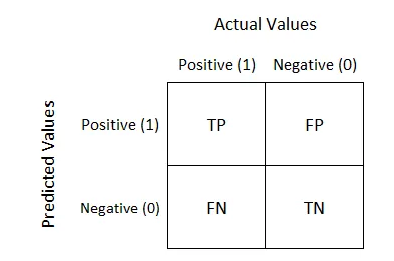
\includegraphics{graphics/confusionmatrix.PNG}
    \caption[Confusion matrix]{Confusion matrix\autocite{Narkhede2018}.
        \label{fig:confusionmatrix}}
\end{figure}
\begin{enumerate}
    \item De accuracy geeft weer hoe goed het model voorspellingen maakt. Dit wordt voorgesteld door het aantal correcte voorspellingen  \autocite{Narkhede2018}.
    \[ \text{Accuracy} = \frac{\text{TP+TN}}{\text{TP+TN+FP+FN}} \]
    
    \item De precision stelt de hoeveelheid correcte positieve voorspellingen voor.
    \[ \text{Precision} = \frac{\text{TP}}{\text{TP+FP}} \]
    
    \item De recall, ook wel sensitivity genoemd, stelt de kans op een positieve klasse voor.  
    \[ \text{Recall} = \frac{\text{TP}}{\text{TP+FN}} \]
    
    \item De specificity, stelt de kans op een negatieve klasse voor.
    \[ \text{Specificity} = \frac{\text{TN}}{\text{TN+FP}} \]
    
    \item De F1-score is het gemiddelde van de precision en recall scores, waarbij 1.0 de maximale score is.
    \[ \text{F1-score} = \frac{\text{2 x Precision x Recall}}{\text{Precision + Recall}} \]
\end{enumerate}

Voor de voorspelling van leeftijd is het ook aangeraden om 2 andere ratios te gebruiken, namelijk True Acceptance Rate (TAR) en False Reject Rate (FRR) \autocite{Othman2014}. Hierdoor krijgen we per leeftijdscategorie een overzicht van het aantal juist en fout voorspelde afbeeldingen. 
\begin{enumerate}
    \item De TAR geeft het aantal juist voorspelde afbeeldingen binnen de opgegeven leeftijdscategorie.
    \[ \text{True Acceptance Rate} = \frac{\text{Juist voorspelde leeftijdscategorie}}{\text{Totale aantal afbeeldingen}} x 100 \]
    \item De FRR geeft het aantal fout voorspelde afbeeldingen binnen de opgegeven leeftijdscategorie.
    \[ \text{False Rejected Rate} = \frac{\text{Fout voorspelde leeftijdscategorie}}{\text{Totale aantal afbeeldingen}}  x 100 \]
\end{enumerate}

